% Options for packages loaded elsewhere
\PassOptionsToPackage{unicode}{hyperref}
\PassOptionsToPackage{hyphens}{url}
\documentclass[
  11pt,
  a4paper,
]{article}
\usepackage{xcolor}
\usepackage[margin=22mm]{geometry}
\usepackage{amsmath,amssymb}
\setcounter{secnumdepth}{-\maxdimen} % remove section numbering
\usepackage{iftex}
\ifPDFTeX
  \usepackage[T1]{fontenc}
  \usepackage[utf8]{inputenc}
  \usepackage{textcomp} % provide euro and other symbols
\else % if luatex or xetex
  \usepackage{unicode-math} % this also loads fontspec
  \defaultfontfeatures{Scale=MatchLowercase}
  \defaultfontfeatures[\rmfamily]{Ligatures=TeX,Scale=1}
\fi
\usepackage{lmodern}
\ifPDFTeX\else
  % xetex/luatex font selection
\fi
% Use upquote if available, for straight quotes in verbatim environments
\IfFileExists{upquote.sty}{\usepackage{upquote}}{}
\IfFileExists{microtype.sty}{% use microtype if available
  \usepackage[]{microtype}
  \UseMicrotypeSet[protrusion]{basicmath} % disable protrusion for tt fonts
}{}
\makeatletter
\@ifundefined{KOMAClassName}{% if non-KOMA class
  \IfFileExists{parskip.sty}{%
    \usepackage{parskip}
  }{% else
    \setlength{\parindent}{0pt}
    \setlength{\parskip}{6pt plus 2pt minus 1pt}}
}{% if KOMA class
  \KOMAoptions{parskip=half}}
\makeatother
\usepackage{graphicx}
\makeatletter
\newsavebox\pandoc@box
\newcommand*\pandocbounded[1]{% scales image to fit in text height/width
  \sbox\pandoc@box{#1}%
  \Gscale@div\@tempa{\textheight}{\dimexpr\ht\pandoc@box+\dp\pandoc@box\relax}%
  \Gscale@div\@tempb{\linewidth}{\wd\pandoc@box}%
  \ifdim\@tempb\p@<\@tempa\p@\let\@tempa\@tempb\fi% select the smaller of both
  \ifdim\@tempa\p@<\p@\scalebox{\@tempa}{\usebox\pandoc@box}%
  \else\usebox{\pandoc@box}%
  \fi%
}
% Set default figure placement to htbp
\def\fps@figure{htbp}
\makeatother
\setlength{\emergencystretch}{3em} % prevent overfull lines
\providecommand{\tightlist}{%
  \setlength{\itemsep}{0pt}\setlength{\parskip}{0pt}}
\usepackage{bookmark}
\IfFileExists{xurl.sty}{\usepackage{xurl}}{} % add URL line breaks if available
\urlstyle{same}
\hypersetup{
  pdftitle={Baker\textquotesingle s theorem II: extrapolation and the end of the proof},
  pdfauthor={GPT-6.1 Sol (OpenAI), Ultra},
  hidelinks,
  pdfcreator={LaTeX via pandoc}}

\title{Baker\textquotesingle s theorem II: extrapolation and the end of
the proof}
\author{GPT-6.1 Sol (OpenAI), Ultra}
\date{October 2026}

\providecommand{\Eta}{\mathrm{H}}
\begin{document}
\maketitle

\emph{Draft. Public domain (CC0).}

The preceding lesson produced a nonzero integer coefficient array. To
finish the proof, we must recover one of those integers from analytic
data and show that its absolute value is below \(1\). We begin by
deriving that recovery problem. It determines how many small derivatives
we need, why close frequencies matter, and how exact zeros must be
extended before Cauchy's formula can help.

We use Propositions 2.2--2.3 from
\href{../TR-BAKER-02.html}{\emph{Baker's theorem I: building an
auxiliary function}} and the height lower bound from
\href{../TR-BAKER-01.html}{\emph{Linear forms in logarithms: the
problem, the trivial bounds, and effectivity}}. Baker's
auxiliary-function and extrapolation method is explained in the freely
accessible {[}Waldschmidt 2003{]} lectures; the coefficient selectors
and all parameter comparisons used here are proved below. The analytic
inputs are the maximum-modulus principle, Cauchy's formula and the chain
rule.

After the proof, we examine how a logarithmic form arises from an
arithmetic expression, and which hypothesis proves that it is nonzero.
For the Dirichlet application,
\href{../../NT-ANT/abelian-number-fields-and-dirichlet-l-functions-at-s-1.html}{\emph{Abelian
number fields and Dirichlet L-functions at \(s=1\)}}, Theorem 17.3 and
its imprimitive-character paragraph, proves \(L(1,\chi)\ne0\). A freely
accessible proof at the same generality is {[}Sutherland 2021{]},
Theorem 19.16, with its preceding class-number and cyclotomic arguments.
The theorem, branches and proof methods retain the human attribution
listed in the references.

\subsection{1. Start with the integer that must be
recovered}\label{start-with-the-integer-that-must-be-recovered}

The contradiction will concern one coefficient, rather than a claim that
an entire function with small derivatives must vanish. After restricting
the function of the preceding lesson to the diagonal, relation (2.1)
gives a finite sum

\[
\phi(z)=\sum_{i=1}^{R}\sum_{k=0}^{S-1}p_{k,i}z^ke^{\xi_i z},
\qquad R=(L+1)^n,\quad S=L+1.
\]

The coefficients are integers and at least one is nonzero. Rational
independence of the original logarithms makes the frequencies distinct.
We will justify their quantitative separation below.

For a polynomial \(W(z)=\sum_jw_jz^j\), differentiation at the origin
gives

\[
\sum_jw_j\left.\frac{d^j}{dz^j}(z^ke^{\xi_i z})\right|_{z=0}
=W^{(k)}(\xi_i).
\]

Indeed, for a monomial \(W(z)=z^j\), both sides are \((j)_k\xi_i^{j-k}\)
if \(j\ge k\), and zero otherwise; linearity proves the identity. If
\(W\) has one prescribed derivative equal to \(1\) and all the other
derivatives through order \(S-1\) equal to zero at these nodes, then the
left side recovers exactly one \(p_{k,i}\).

This tells us what the analytic part has to deliver. With \(N=RS\), it
is enough to bound the first \(N\) derivatives by \(\varepsilon\),
construct a selector of degree below \(N\) with coefficients at most
\(M\), and arrange \(NM\varepsilon<1\). The nonzero recovered integer
would then have absolute value below \(1\). The next two sections
construct and bound the selector; Sections 4--6 produce the required
derivatives.

\subsubsection{A four-dimensional selector
calculation}\label{a-four-dimensional-selector-calculation}

Take two nodes \(0,1\), each with two prescribed derivatives. For

\[
\psi(z)=p_{0,0}+p_{1,0}z+(p_{0,1}+p_{1,1}z)e^z,
\]

the polynomial \(W_0(z)=1-3z^2+2z^3\) has value \(1\) at \(0\), and has
zero derivative there and zero value and derivative at \(1\). Therefore

\[
p_{0,0}=\psi(0)-3\psi''(0)+2\psi'''(0).
\]

Similarly \(W_1(z)=z-2z^2+z^3\) selects the first derivative at \(0\),
giving

\[
p_{1,0}=\psi'(0)-2\psi''(0)+\psi'''(0).
\]

If \(p_{0,0}\) is a nonzero integer and these derivatives all have size
below \(1/6\), the first identity is impossible. This is an example of
the interpolation calculation itself; the general Baker proof uses its
actual logarithmic nodes and the uniform selector bound below. In
particular, it must be able to select whichever coefficient is nonzero.

\subsection{2. Separate the frequencies}\label{separate-the-frequencies}

On the diagonal, relation (2.1) turns the auxiliary function into

\[
\phi(z)=\sum_{\lambda_1,\ldots,\lambda_n=0}^{L}
\left(\sum_{s=0}^{L}p_{s,\lambda_1,\ldots,\lambda_n}z^s\right)e^{\xi_\lambda z},
\qquad \xi_\lambda=\sum_{j=1}^n\lambda_j\ell_j. \tag{3.11}
\]

Rational independence makes these \((L+1)^n\) frequencies distinct. For
coefficient recovery, very close frequencies would make the
interpolation coefficients too large. Elementary arithmetic gives the
needed separation.

\textbf{Lemma 3.3 (frequency separation).} There is a constant \(c>1\),
depending only on the fixed algebraic numbers and logarithms, such that,
for every integer \(T\ge1\) and every nonzero integer vector \(t\) with
\(|t_j|\le T\),

\[
\left|\sum_jt_j\ell_j\right|>c^{-T}. \tag{3.12}
\]

\textbf{Proof.} Put \(\Omega=\sum_jt_j\ell_j\ne0\) and \(P=e^\Omega\).
If \(P=1\), then \(\Omega\) is a nonzero multiple of \(2\pi i\), so
\(|\Omega|\ge2\pi\). This case must be kept: rational independence of
arbitrary complex logarithms does not assert multiplicative independence
of their bases.

If \(P\ne1\), Proposition 1.3 gives

\[
|P-1|\ge\exp\left(-D\log2-DT\sum_jh(\alpha_j)\right),
\qquad D=[\mathbb Q(\alpha_1,\ldots,\alpha_n):\mathbb Q].
\]

If \(|\Omega|\le1/2\), Lemma 1.1 gives \(|P-1|\le2|\Omega|\), hence
\(|\Omega|\ge e^{-CT}\) for a fixed \(C>0\). If \(|\Omega|>1/2\),
enlarge \(C\) to get the same conclusion. Choose \(c>e^C\) to make the
inequality strict in every case. \(\square\)

For the frequencies in (3.11), define

\[
\sigma=\max(1,\max_\lambda|\xi_\lambda|),\qquad
\rho=\min(1,\min_{\lambda\ne\mu}|\xi_\lambda-\xi_\mu|).
\]

Differences have integer coefficients bounded by \(L\), so
\(\sigma\le C_4(L+1)\) and \(\rho>c^{-L}\). This exponentially small
separation is sufficient.

\subsection{3. Build and bound the coefficient
selector}\label{build-and-bound-the-coefficient-selector}

\textbf{Lemma 3.4 (Hermite selector).} Let \(\xi_1,\ldots,\xi_R\) be
distinct complex numbers, \(S\ge1\), and define

\[
\sigma=\max(1,|\xi_1|,\ldots,|\xi_R|),\qquad
\rho=\min(1,\min_{i\ne j}|\xi_i-\xi_j|).
\]

For \(R=1\), set \(\rho=1\). Given \(1\le t\le R\), \(0\le s<S\), there
is a polynomial \(W(z)=\sum_{j=0}^{RS-1}w_jz^j\) with

\[
W^{(k)}(\xi_i)=\begin{cases}1,&(i,k)=(t,s),\\0,&\text{otherwise},\end{cases}
\quad 1\le i\le R,\quad 0\le k<S,
\]

and

\[
|w_j|\le(8\sigma/\rho)^{RS}. \tag{3.13}
\]

\textbf{Proof.} For \(R\ge2\), put \(V(z)=\prod_{i\ne t}(z-\xi_i)^S\),
\(M=(R-1)S\), and expand

\[
\frac1{V(\xi_t+x)}=\sum_{j\ge0}c_jx^j.
\]

Define

\[
W(z)=\frac{(z-\xi_t)^s}{s!}\,V(z)
\sum_{j=0}^{S-1-s}c_j(z-\xi_t)^j. \tag{3.14}
\]

Its degree is at most \(M+s+S-1-s=RS-1\). The factor \(V\) forces order
\(S\) at every other node. At \(\xi_t\), reciprocal truncation gives
\(W(\xi_t+x)=x^s/s!+O(x^S)\), proving the prescribed derivatives.

For the size bound, regard \(V(\xi_t+x)\) as a product of \(M\) linear
factors, counting repetitions. Each constant term has size at least
\(\rho\). Multiplying their reciprocal geometric series gives

\[
|c_j|\le\binom{M+j-1}{j}\rho^{-(M+j)}.
\]

For \(j\le S-1-s\), \(M+j<RS\), and \(\binom{M+j-1}{j}\le2^{M+j}\). Thus
\(|c_j|\le(2/\rho)^{RS}\). The sum of absolute values of the
coefficients of \(V(z)(z-\xi_t)^{s+j}\) is at most

\[
\prod_{i\ne t}(1+|\xi_i|)^S(1+|\xi_t|)^{s+j}\le(2\sigma)^{RS}.
\]

There are at most \(S\) terms in (3.14), and \(1/s!\le1\). Every
coefficient is therefore at most \(S(4\sigma/\rho)^{RS}\). Since
\(S\le2^{RS}\), this implies (3.13). For \(R=1\), take
\(W(z)=(z-\xi_1)^s/s!\); its coefficient sum is at most \((2\sigma)^S\),
also within the stated bound. \(\square\)

The normalization matters. A polynomial equal to \((z-\xi_t)^s\) to
order \(S\) would select \(s!\) times the desired coefficient. The
factor \(1/s!\) selects the coefficient itself.

\subsection{4. The family on which zeros can be
transferred}\label{the-family-on-which-zeros-can-be-transferred}

Suppose that the algebraic logarithms \(\ell_1,\ldots,\ell_n\) are
rationally independent but that \(1,\ell_1,\ldots,\ell_n\) satisfy an
algebraic-coefficient relation. Use the normalization and the function
\(\Phi\) of the preceding lesson. Put

\[
a=\frac1{8n},\qquad L=\lfloor h^{2-2a}\rfloor,\qquad
f_m(z)=\partial^m\Phi(z,\ldots,z).
\]

For all sufficiently large integers \(h\), its integer coefficients
\(p_\lambda\), not all zero, satisfy \(|p_\lambda|\le e^{h^3}\). We have

\[
f_m(l)=0\quad(1\le l\le h,\ |m|\le h^2), \tag{3.1}
\]

and, for every \(|m|\le h^2\),

\[
|f_m(z)|\le e^{C_2(h^3+L|z|)}. \tag{3.2}
\]

At every positive integer \(l\), either \(f_m(l)=0\) or

\[
|f_m(l)|\ge e^{-C_3(h^3+Ll)}. \tag{3.3}
\]

The same \(C_2,C_3\) work for every permitted derivative. They depend on
the fixed algebraic relation and its logarithms, but never on
\(h,m,l,z\). This uniformity permits a finite sequence of
extrapolations.

When differentiating along the diagonal, we use

\[
\frac{d^k}{dz^k}f_m(z)
=\sum_{j_0+\cdots+j_{n-1}=k}
\frac{k!}{j_0!\cdots j_{n-1}!}\,\partial^{m+j}\Phi(z,\ldots,z). \tag{3.4}
\]

This is the repeated chain rule for the operator
\(\partial_{z_0}+\cdots+\partial_{z_{n-1}}\). Thus vanishing of
multivariable derivatives through total order \(S\) implies that \(f_m\)
has a zero of order at least \(S-|m|+1\) at the same diagonal point.

\subsubsection{The exact-zero transfer
contract}\label{the-exact-zero-transfer-contract}

The analytic and arithmetic estimates can be compared before choosing
Baker's particular powers of \(h\). The following elementary statement
identifies the quantity that an extrapolation step needs to make
positive.

\textbf{Lemma (one extrapolation step).} Let \(R,S,Q\) be positive
integers with \(Q\ge R\). Let \(f\) be entire and have a zero of order
at least \(S\) at every integer \(1,\ldots,R\). Suppose that, for
nonnegative constants \(U,V,A,B\),

\[
|f(z)|\le e^{U+V|z|},
\]

and at each integer \(1\le l\le Q\) either \(f(l)=0\) or
\(|f(l)|\ge e^{-A-Bl}\). If a radius \(\mathcal R>Q\) satisfies

\[
RS\log\frac{\mathcal R-R}{Q}
>U+V\mathcal R+A+BQ,
\]

then \(f(l)=0\) for every integer \(1\le l\le Q\).

\textbf{Proof.} Put \(F(z)=\prod_{r=1}^{R}(z-r)^S\). The quotient
\(f/F\) is entire because the prescribed zeros remove its apparent
poles. On \(|z|=\mathcal R\), we have \(|F(z)|\ge(\mathcal R-R)^{RS}\).
For a new integer \(R<l\le Q\), we have \(|F(l)|\le Q^{RS}\). The
maximum-modulus principle consequently gives

\[
\log|f(l)|\le U+V\mathcal R
-RS\log\frac{\mathcal R-R}{Q}
<-A-BQ\le-A-Bl
\]

if \(f(l)\ne0\). This contradicts the arithmetic lower bound. The old
integers already have zero values by hypothesis. \(\square\)

The factor \(RS\) measures how many exact zeros, counted with
multiplicity, are available for division. The logarithm measures the
gain from comparing the outer circle with the new interval. The two
growth budgets on the right measure what that gain must defeat. Small
initial values would not give an entire quotient, so they cannot replace
the exact-zero hypothesis.

For the family \(f_m\), the chain rule (3.4) supplies the multiplicity.
We keep derivative indices through \(S_{J+1}\) and spend another
\(S_{J+1}\) orders on division. Thus \(2S_{J+1}\le S_J\) is a sufficient
budget rule. In the next proposition use

\[
\begin{gathered}
R=R_J,\quad S=S_{J+1},\quad Q=R_{J+1},\quad
\mathcal R=R_{J+1}h^a,\\
U=C_2h^3,\quad V=C_2L,\quad
A=C_3h^3,\quad B=C_3L.
\end{gathered}
\]

The computations (3.7)--(3.8) verify this contract simultaneously for
the fixed number of steps. They are what makes the particular schedule
work; the schedule alone is not a proof that new zeros appear.

\subsection{5. Verify the transfer
schedule}\label{verify-the-transfer-schedule}

Define, for \(0\le J\le J_*=(8n)^2\),

\[
R_J=\left\lfloor h^{1+Ja}\right\rfloor,\qquad
S_J=\left\lfloor\frac{h^2}{2^J}\right\rfloor.
\]

The number of points grows, while the derivative budget is halved at
each step. The number of steps is fixed once \(n\) is fixed. We may
therefore choose \(h\) large enough for every estimate at every step
simultaneously.

\textbf{Proposition 3.1 (extrapolation).} For all sufficiently large
integers \(h\),

\[
\partial^m\Phi(l,\ldots,l)=0
\quad(1\le l\le R_J,\ |m|\le S_J,\ 0\le J\le J_*). \tag{3.5}
\]

\textbf{Proof.} The case \(J=0\) is (3.1). Suppose the assertion holds
at \(J<J_*\), and fix \(|m|\le S_{J+1}\). Formula (3.4) shows that the
derivatives of \(f_m\) of orders \(0,\ldots,S_{J+1}-1\) vanish at
\(1,\ldots,R_J\). Their total multivariable orders are at most

\[
|m|+S_{J+1}-1<2S_{J+1}\le S_J;
\]

the last inequality follows from
\(2\lfloor x/2\rfloor\le\lfloor x\rfloor\). Consequently

\[
F(z)=\prod_{r=1}^{R_J}(z-r)^{S_{J+1}}
\]

divides \(f_m\) as an entire function: all apparent poles of \(f_m/F\)
are removable.

Take the circle of radius \(\mathcal R=R_{J+1}h^a\). For sufficiently
large \(h\), \(h^a\ge2\), so \(\mathcal R-R_J\ge\mathcal R/2\). On the
circle,

\[
|F(z)|\ge(\mathcal R/2)^{R_JS_{J+1}}.
\]

At a new integer \(R_J<l\le R_{J+1}\), every \(|l-r|\le R_{J+1}\), so
\(|F(l)|\le R_{J+1}^{R_JS_{J+1}}\). Apply the maximum-modulus principle
to \(f_m/F\), and use (3.2). If \(f_m(l)\ne0\), then

\[
\log|f_m(l)|\le C_2(h^3+L\mathcal R)
-R_JS_{J+1}(a\log h-\log2). \tag{3.6}
\]

We check the powers explicitly. Once the quantities being rounded are at
least \(2\),

\[
R_JS_{J+1}\ge\frac{h^{3+Ja}}{2^{J+3}},\qquad
L\mathcal R\le h^{2-2a}h^{1+(J+1)a}h^a=h^{3+Ja}.
\]

Also \(h^3\le h^{3+Ja}\), hence

\[
h^3+L\mathcal R\le 2^{J+4}R_JS_{J+1}. \tag{3.7}
\]

The arithmetic alternative (3.3) would require

\[
\log|f_m(l)|\ge-C_3(h^3+Ll)\ge-C_3(h^3+L\mathcal R).
\]

This contradicts (3.6)--(3.7) whenever

\[
a\log h-\log2>(C_2+C_3)2^{J+4}. \tag{3.8}
\]

There are only \(J_*\) induction steps. Choose \(h\) so that all the
rounding bounds and (3.8) hold for every \(J<J_*\). Every new integer
value is then zero; the old ones vanish by the induction hypothesis.
This proves (3.5). \(\square\)

The proof uses exact zeros twice. Multiplicity allows division by \(F\);
arithmetic converts the resulting small values into new exact zeros.
Merely small initial derivatives would not justify the same division.

\begin{minipage}[t]{\linewidth}
\centering
\pandocbounded{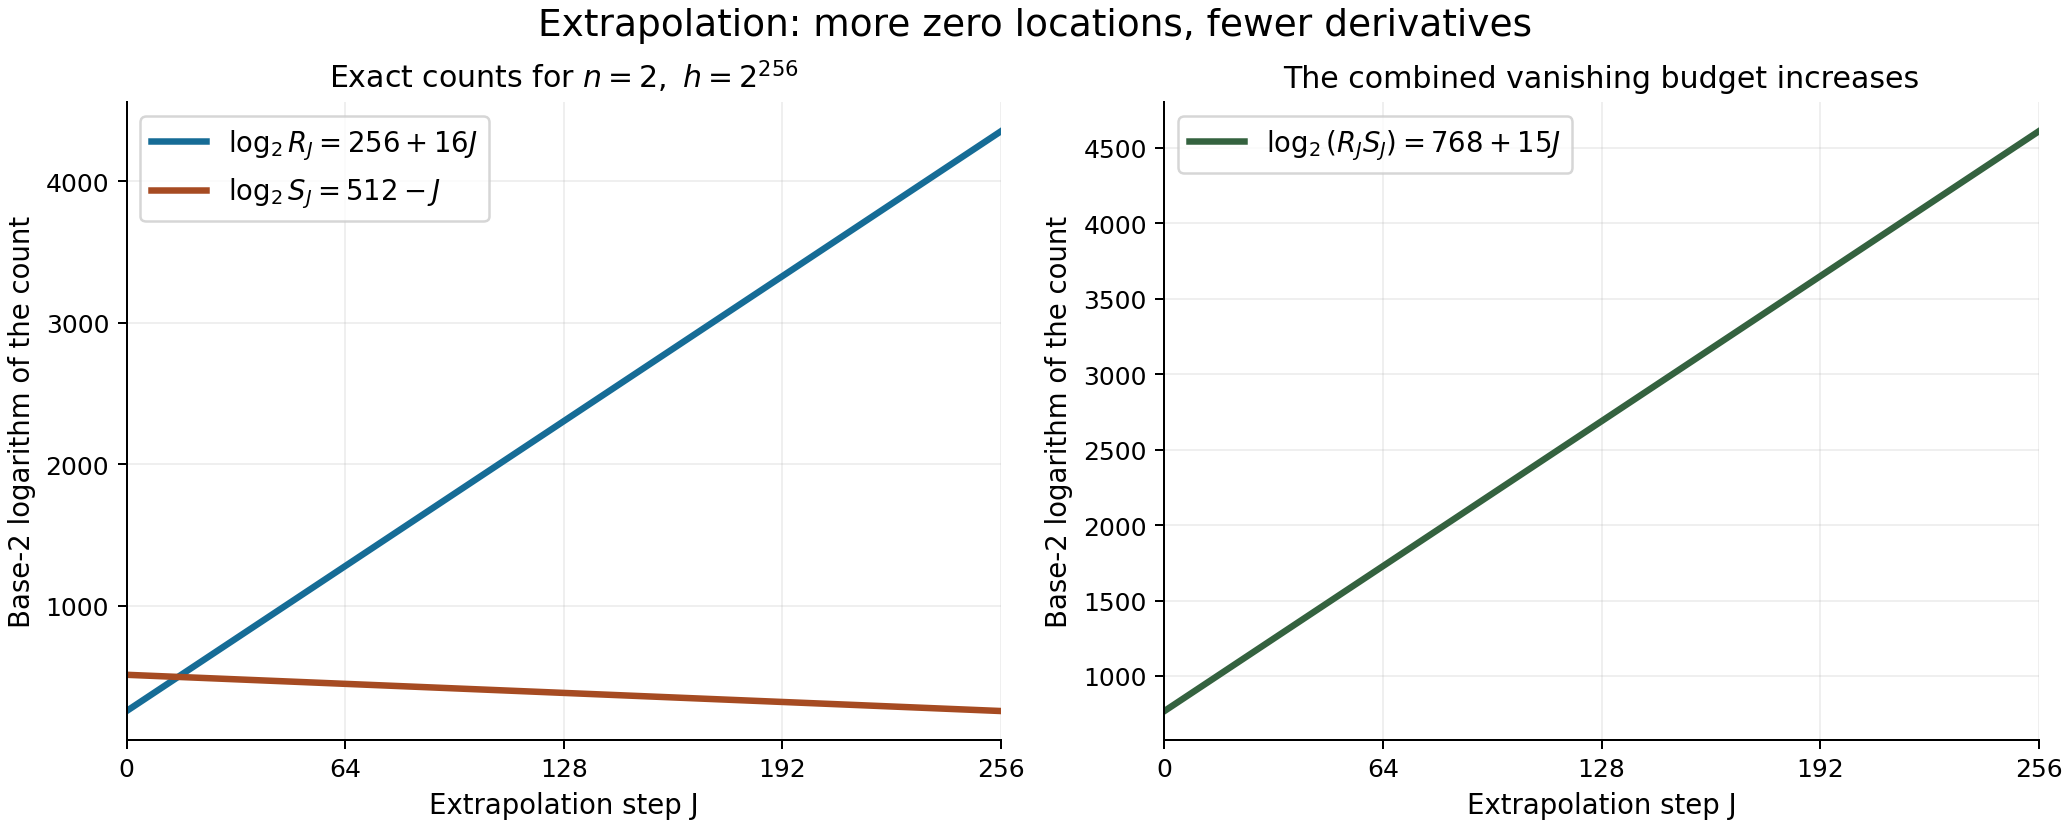
\includegraphics[keepaspectratio,alt={The number of zero locations grows faster than the derivative budget decreases.}]{../figures/extrapolation-budget.png}}
\par\smallskip
\begin{flushleft}\small
\emph{Figure 1. Exact parameter counts for \(n=2\), \(h=2^{256}\) and
\(0\le J\le256\): \(\log_2 R_J=256+16J\), \(\log_2 S_J=512-J\), and
\(\log_2(R_JS_J)=768+15J\). This displays the growth mechanism of
Proposition 3.1. These values illustrate the counts; they are not a
universal threshold for \(C_2,C_3\). The reproducible source accompanies
the lesson.}
\end{flushleft}
\end{minipage}\par\medskip


\subsection{6. Reach the derivative budget for coefficient
recovery}\label{reach-the-derivative-budget-for-coefficient-recovery}

Write

\[
\phi(z)=\Phi(z,\ldots,z),\qquad
X=h^{8n},\qquad Y=\left\lfloor\frac{h^2}{2^{J_*}}\right\rfloor.
\]

Since \(R_{J_*}=h^{1+8n}\ge X\), Proposition 3.1 and (3.4) show that
\(\phi\) vanishes to order at least \(Y\) at each integer
\(1,\ldots,X\). Here \(X\) is an integer. The fixed factor \(2^{J_*}\)
may be enormous, but \(Y\to\infty\) as \(h\to\infty\).

\textbf{Proposition 3.2 (derivatives at the origin).} For all
sufficiently large integers \(h\),

\[
|\phi^{(j)}(0)|<e^{-h^{8n}}\qquad(0\le j\le h^{8n}). \tag{3.9}
\]

\textbf{Proof.} Set \(E(z)=\prod_{r=1}^{X}(z-r)^Y\) and
\(\mathcal R=Xh^a\). The quotient \(\phi/E\) is entire. On
\(|z|=\mathcal R\), \(|E(z)|\ge(\mathcal R/2)^{XY}\) for large \(h\). On
\(|w|\le1\), \(|E(w)|\le(2X)^{XY}\). The growth bound and
maximum-modulus principle give

\[
\sup_{|w|\le1}|\phi(w)|\le
\exp\!\left(C_2(h^3+L\mathcal R)-XY(a\log h-\log4)\right). \tag{3.10}
\]

For large \(h\), \(Y\ge h^2/2^{J_*+1}\), and therefore

\[
\frac{L\mathcal R}{XY}\le 2^{J_*+1}h^{-a}\longrightarrow0,\qquad
\frac{h^3}{XY}\le2^{J_*+1}h^{1-8n}\longrightarrow0.
\]

The positive term in (3.10), divided by \(XY\), tends to zero, whereas
\(a\log h-\log4\) tends to infinity. Thus the supremum is at most
\(e^{-XY}\) eventually. Cauchy's formula on the unit circle yields
\(|\phi^{(j)}(0)|\le j!e^{-XY}\). For \(j\le X\),
\(\log(j!)\le X\log X\). Since \(Y>\log X+1\) eventually, this is
strictly less than \(e^{-X}\), proving (3.9). \(\square\)

Small derivatives alone do not imply that an entire function is zero.
The number of frequencies and the degree of its polynomial coefficients
must now enter the argument.

\subsection{7. Recover the integer and
conclude}\label{recover-the-integer-and-conclude}

Set \(S=L+1\), \(R=(L+1)^n\) and \(N=RS=(L+1)^{n+1}\). Choose a nonzero
integer coefficient \(p_{s,t}\) in (3.11), and let \(W\) be its
selector. For \(s\ge0\),

\[
\left.\frac{d^j}{dz^j}(z^se^{\xi z})\right|_{z=0}
=\frac{d^s}{d\xi^s}\xi^j.
\]

Both sides are zero for \(j<s\), and otherwise equal \((j)_s\xi^{j-s}\).
Multiply by \(w_j\) and sum. The selector conditions give the exact
coefficient identity

\[
\sum_{j=0}^{N-1}w_j\phi^{(j)}(0)
=\sum_{i=1}^R\sum_{k=0}^{S-1}p_{k,i}W^{(k)}(\xi_i)
=p_{s,t}. \tag{3.15}
\]

All needed derivative orders fit inside Proposition 3.2, since

\[
N\le2^{n+1}h^{2n+2}=o(h^{8n})\qquad(n\ge1).
\]

The frequency bounds and (3.13) yield

\[
\log\max_j|w_j|
\le N\bigl(\log(8C_4(L+1))+L\log c\bigr)\le C_5h^{2n+4}
\]

for large \(h\). In particular \(2n+4<8n\), even for \(n=1\). Combining
(3.9) and (3.15) gives

\[
1\le|p_{s,t}|\le N\exp(C_5h^{2n+4}-h^{8n})<1
\]

eventually. The first inequality holds because the selected coefficient
is a nonzero integer. This contradiction rules out the original
relation.

We have proved \textbf{Baker's theorem}: arbitrary rationally
independent logarithms of nonzero algebraic numbers remain linearly
independent over \(\overline{\mathbb Q}\) after adjoining \(1\). The
proof does not require multiplicative independence, positive bases, or
principal branches.

\subsection{8. Additive forms: find the source of
nonvanishing}\label{additive-forms-find-the-source-of-nonvanishing}

The theorem about independent logarithms gives an especially useful rule
for arbitrary, possibly dependent logarithms: first reduce to a rational
basis, then ask whether the resulting form is zero. The zero case must
be handled by the application, because Baker's theorem permits it.

\textbf{Corollary 3.5.} For nonzero algebraic \(\alpha_j\), chosen
logarithms \(\ell_j\), and algebraic \(\beta_j\), the homogeneous form
\(H=\sum_j\beta_j\ell_j\) is either zero or transcendental.

\textbf{Proof.} Select a rational basis \(\kappa_1,\ldots,\kappa_r\)
from the logarithms spanning them, and rewrite
\(H=\sum_k\eta_k\kappa_k\), with algebraic \(\eta_k\). A nonzero
algebraic \(H\) would give the nontrivial relation
\(-H+\sum_k\eta_k\kappa_k=0\), contradicting independence of
\(1,\kappa_1,\ldots,\kappa_r\). If the span is zero, \(H=0\) directly.
\(\square\)

Thus \(\beta_0+H\), with algebraic \(\beta_0\), is transcendental
whenever \(H\ne0\); if \(H=0\), its value is the algebraic number
\(\beta_0\). Nonvanishing of the entire inhomogeneous expression is
insufficient: \(\beta_0=1\) with all logarithmic coefficients zero gives
\(1\). This qualification belongs in the statement.

\subsubsection{\texorpdfstring{Dirichlet \(L\)-values as logarithmic
forms}{Dirichlet L-values as logarithmic forms}}\label{dirichlet-l-values-as-logarithmic-forms}

Let \(\chi\) be a nonprincipal Dirichlet character modulo \(q>1\),
extended by zero off the units. Put \(\zeta=e^{2\pi i/q}\) and

\[
\widehat\chi(m)=\frac1q\sum_{r=1}^q\chi(r)\zeta^{-mr}\quad(0\le m<q).
\]

Character values are zero or roots of unity, so these coefficients are
algebraic. Multiplication of the residues by a unit on which
\(\chi\ne1\) proves that its period sum is zero, hence
\(\widehat\chi(0)=0\). Finite geometric sums give Fourier inversion:

\[
\chi(n)=\sum_{m=1}^{q-1}\widehat\chi(m)\zeta^{mn}. \tag{3.16}
\]

The partial sums of \(\chi(n)\) are bounded by periodicity and the zero
period sum. Summation by parts therefore proves convergence of
\(\sum_{n\ge1}\chi(n)/n\). To justify the logarithmic identity, first
insert \(0<t<1\). Absolute convergence and (3.16) give

\[
\sum_{n\ge1}\frac{\chi(n)t^n}{n}
=-\sum_{m=1}^{q-1}\widehat\chi(m)\operatorname{Log}(1-t\zeta^m). \tag{3.17}
\]

The power series for \(-\operatorname{Log}(1-z)\) follows by integrating
the geometric series. The path \(1-t\zeta^m\) stays in the right
half-plane, so its logarithm is principal.

We also supply the limiting argument. If \(\sum a_n=S\) converges and
\(A_N=\sum_{n\le N}a_n\), summation by parts gives

\[
\sum_{n\ge1}a_nt^n=(1-t)\sum_{N\ge1}A_Nt^N\longrightarrow S\quad(t\uparrow1).
\]

Replace \(A_N\) by \(S+(A_N-S)\). The constant part tends to \(S\). Any
fixed initial error segment tends to zero, while its tail is bounded by
\(\sup_{N\ge N_0}|A_N-S|\). Apply this to \(a_n=\chi(n)/n\). For
\(1\le m<q\), \(1-\zeta^m\ne0\) has positive real part, so (3.17) tends
to

\[
L(1,\chi)=-\sum_{m=1}^{q-1}\widehat\chi(m)\operatorname{Log}(1-\zeta^m). \tag{3.18}
\]

Theorem 17.3 of the internal \emph{Number fields} lesson cited in the
introduction proves nonvanishing for primitive nontrivial characters.
Its following paragraph covers imprimitive characters by the nonzero
Euler factors \(1-\chi^*(p)/p\). Thus (3.18) is a nonzero homogeneous
algebraic-coefficient logarithmic form. Corollary 3.5 proves:

\textbf{Theorem 3.9.} For every nonprincipal Dirichlet character modulo
\(q>1\), \(L(1,\chi)\) is transcendental.

For \(\chi_4\), whose values at \(1,3\pmod4\) are \(1,-1\), the only
nonzero Fourier coefficients are \(\widehat\chi_4(1)=-i/2\),
\(\widehat\chi_4(3)=i/2\). Hence

\[
L(1,\chi_4)=\frac i2\bigl(\operatorname{Log}(1-i)-\operatorname{Log}(1+i)\bigr)=\frac\pi4.
\]

The real parts cancel; the arguments are \(-\pi/4\) and \(\pi/4\). This
checks the Fourier sign and the branch convention.

\subsubsection{A modulus and its induced
character}\label{a-modulus-and-its-induced-character}

The Fourier identity also shows why one must preserve the nonvanishing
input when passing to an imprimitive modulus. Let \(\chi_3(1)=1\),
\(\chi_3(2)=-1\), extended periodically and by zero at multiples of
\(3\). Its Fourier coefficients at \(m=1,2\) are \(-i/\sqrt3,i/\sqrt3\).
If \(\zeta=e^{2\pi i/3}\), then

\[
L(1,\chi_3)=\frac{i}{\sqrt3}
\bigl(\operatorname{Log}(1-\zeta)-\operatorname{Log}(1-\zeta^2)\bigr).
\]

The two arguments are \(-\pi/6\) and \(\pi/6\), and both moduli equal
\(\sqrt3\). The real parts cancel, so \(L(1,\chi_3)=\pi/(3\sqrt3)\).
This value is nonzero; it checks both the Fourier sign and the selected
logarithmic branches.

Now let \(\chi_6\) be the character modulo \(6\) induced by \(\chi_3\).
The terms removed from the \(\chi_3\)-series are exactly the even ones.
For their convergent sum,

\[
\sum_{k\ge1}\frac{\chi_3(2k)}{2k}
=-\frac12L(1,\chi_3).
\]

Consequently \(L(1,\chi_6)=\tfrac32L(1,\chi_3)=\pi/(2\sqrt3)\). This is
the Euler factor \(1-\chi_3(2)/2\) in a concrete instance. The general
nonvanishing theorem, rather than this example, supplies the
corresponding conclusion at every nonprincipal modulus.

\subsection{9. Products and branch
tests}\label{products-and-branch-tests}

A product of powers requires a different check from an additive form: an
assumed algebraic product supplies one more algebraic base, whose
logarithm can be chosen to be the entire exponent. There is no need to
replace each original branch by a principal branch. Two hypotheses make
this procedure useful: independence of the exponents, or a nonzero
algebraic exponential factor. We treat those mechanisms separately.

\subsubsection{Independent exponents}\label{independent-exponents}

\textbf{Corollary 3.7.} Suppose all \(\alpha_j\) are algebraic and
different from \(0,1\), and \(1,\beta_1,\ldots,\beta_n\) are rationally
independent algebraic numbers. Then every chosen value of
\(\prod_j\alpha_j^{\beta_j}\) is transcendental.

\textbf{Proof.} If its value \(\gamma\) were algebraic, choose
\(\ell_\gamma=\sum_j\beta_j\ell_j\). Select a rational basis
\(\kappa_k\) of the span of all these logarithms, and write

\[
\ell_\gamma=\sum_kr_{0k}\kappa_k,\qquad
\ell_j=\sum_kr_{jk}\kappa_k,\qquad r_{jk}\in\mathbb Q.
\]

Baker's theorem implies \(r_{0k}-\sum_j\beta_jr_{jk}=0\) for every
\(k\). Independence of \(1,\beta_1,\ldots,\beta_n\) forces all
\(r_{jk}\), including \(r_{0k}\), to vanish. All \(\ell_j\) would be
zero, impossible since \(\alpha_j\ne1\). This also covers \(\gamma=1\).
\(\square\)

For example, \(2^{\sqrt2}3^{\sqrt3}\) is transcendental. If
\(a+b\sqrt2+c\sqrt3=0\) with rational coefficients and \(c\ne0\),
squaring gives \(ab=0\); the resulting possibilities would make
\(\sqrt3\) or \(\sqrt{3/2}\) rational unless all coefficients vanish.
Both are irrational by prime factorization. If \(c=0\), irrationality of
\(\sqrt2\) finishes the check.

\subsubsection{A nonzero algebraic exponential
factor}\label{a-nonzero-algebraic-exponential-factor}

\textbf{Corollary 3.6.} If \(\beta_0\ne0\) is algebraic, every
\(\alpha_j\ne0\) and \(\beta_j\) is algebraic, and powers are defined by
chosen logarithms, then

\[
e^{\beta_0}\alpha_1^{\beta_1}\cdots\alpha_n^{\beta_n}
\]

is transcendental.

\textbf{Proof.} If its value were algebraic \(\gamma\), choose the
logarithm \(\ell_\gamma=\beta_0+\sum_j\beta_j\ell_j\). Then
\(\ell_\gamma-\sum_j\beta_j\ell_j=\beta_0\) is a nonzero algebraic
homogeneous form in logarithms of algebraic numbers, contradicting
Corollary 3.5. This chosen logarithm handles the branches without a
suppressed period term. \(\square\)

\subsubsection{Keeping a period in the nonvanishing
test}\label{keeping-a-period-in-the-nonvanishing-test}

\textbf{Corollary 3.8.} For every algebraic \(\alpha\ne0\), every value
of \(\pi+\log\alpha\) is transcendental. If \(u,v\) are algebraic and
\(v\ne0\), then \(e^{u\pi+v}\) is transcendental.

\textbf{Proof.} Take \(\log(-1)=i\pi\), so
\(\pi+\ell_\alpha=\ell_\alpha-i\log(-1)\). This form is nonzero.
Otherwise \(\ell_\alpha=-\pi\), and the nonzero real number \(-\pi\) and
imaginary number \(i\pi\) would be rationally independent logarithms of
algebraic numbers satisfying the displayed algebraic relation, contrary
to Baker's theorem. Apply Corollary 3.5. For the second assertion, write
\(e^{u\pi+v}=e^v(-1)^{-iu}\) and apply Corollary 3.6. \(\square\)

Here are two boundary checks for the product criteria. First,

\[
2^{\sqrt2}4^{-\sqrt2/2}=1
\]

for the real logarithms. The exponents together with \(1\) are
rationally dependent, so Corollary 3.7 does not apply. Second, setting
\(\beta_0=0\) in Corollary 3.6 would allow the same value \(1\); its
nonzero-constant hypothesis is necessary for that conclusion. These
checks explain the conditions without imposing multiplicative
independence on the bases. The Gelfond--Schneider deduction in the
preceding lesson is now unconditional.

\subsection{10. Exercises}\label{exercises}

\textbf{Exercise 1 (easy).} Prove Corollary 3.8 for arbitrary chosen
logarithms, including \(\alpha=1\). Explain why adding an algebraic
constant to a homogeneous form requires a condition on its logarithmic
part.

\textbf{Exercise 2 (medium).} Prove Lemma 3.3 by a norm argument.
According to the sign of \(t_j\), choose the positive leading
coefficient \(a_j\) of the primitive minimal polynomial of \(\alpha_j\)
or \(\alpha_j^{-1}\), and use

\[
w=\left(\prod_ja_j^{|t_j|}\right)\left(\prod_j\alpha_j^{t_j}-1\right).
\]

Explain separately the case \(w=0\) and the role of rational
independence there.

\textbf{Exercise 3 (medium).} Put \(U(z)=\prod_i(z-\xi_i)^S\), and let
\(C_t\) be a small positively oriented circle around \(\xi_t\)
containing no other node. Show that, for \(z\) outside the circle,

\[
W(z)=\frac{U(z)}{s!\,2\pi i}\int_{C_t}
\frac{(\zeta-\xi_t)^s}{(z-\zeta)U(\zeta)}\,d\zeta
\]

equals (3.14). Deduce its jets and bound (3.13).

\textbf{Exercise 4 (medium).} Prove (3.18), including convergence,
branch choice and nonvanishing for an imprimitive nonprincipal
character. Compute the Fourier coefficients for \(\chi_4\).

\textbf{Exercise 5 (hard).} Prove Corollary 3.7 by induction. First
prove that \(\sum_j\beta_j\ell_j\ne0\) if the algebraic \(\beta_j\) are
rationally independent and all \(\alpha_j\ne0,1\). Handle explicitly an
assumed algebraic product value equal to \(1\).

\textbf{Exercise 6 (hard).} Check every power and rounding bound in
Propositions 3.1--3.2. Explain why \(J_*\) does not prevent
\(Y\to\infty\), and why coefficient recovery works for \(n=1\).

\subsection{11. Solutions}\label{solutions}

\textbf{Solution 1.} The expression \(\ell_\alpha-i\log(-1)\) is
homogeneous. If zero, its two logarithms would be \(-\pi\) and \(i\pi\),
which are rationally independent, contradicting Baker's theorem.
Corollary 3.5 makes its nonzero value transcendental. For \(\alpha=1\),
a chosen logarithm is \(2\pi ik\), giving \((1+2ik)\pi\ne0\), consistent
with the proof. If \(H\ne0\), an algebraic \(\beta_0+H\) would make
\(H\) algebraic after subtraction. If \(H=0\), its value is simply
\(\beta_0\). The exponential assertion follows from \(u\pi=-iu\log(-1)\)
and the nonzero constant \(v\).

\textbf{Solution 2.} If \(a\eta^d+A_1\eta^{d-1}+\cdots+A_d=0\), then
\(a\eta\) satisfies the monic integer polynomial \[
X^d+A_1X^{d-1}+aA_2X^{d-2}+\cdots+a^{d-1}A_d.
\] Thus every \(a_j\alpha_j^{\operatorname{sgn}(t_j)}\), and therefore
\(w\), is an algebraic integer. Omit indices with \(t_j=0\). Each
conjugate of \(w\) has size at most \(e^{CT}\), because the conjugates
of the fixed bases and inverses form a finite list. If \(w\ne0\), its
integer norm gives \(|w|\ge e^{-C(D-1)T}\). Dividing by
\(\prod a_j^{|t_j|}\le e^{C'T}\) bounds \(|P-1|\) below by
\(e^{-C''T}\). If \(|\Omega|\le1/2\), use \(|P-1|\le2|\Omega|\);
otherwise \(|\Omega|>1/2\) already suffices. If \(w=0\), \(P=1\) and
\(\Omega\in2\pi i\mathbb Z\). Independence and \(t\ne0\) exclude zero,
leaving \(|\Omega|\ge2\pi\). Without independence this last exclusion
would fail.

\textbf{Solution 3.} Write \(x=\zeta-\xi_t\),
\(U(\zeta)=x^SV(\xi_t+x)\), and expand \(1/V(\xi_t+x)=\sum c_jx^j\). On
a sufficiently small circle, \[
\frac1{z-\zeta}=\sum_{k\ge0}\frac{x^k}{(z-\xi_t)^{k+1}}.
\] The integral selects the coefficient of \(x^{-1}\), giving \[
\frac{U(z)}{s!}\sum_{j=0}^{S-1-s}
\frac{c_j}{(z-\xi_t)^{S-s-j}}
=\frac{V(z)}{s!}\sum_{j=0}^{S-1-s}c_j(z-\xi_t)^{s+j}.
\] This is (3.14) and extends polynomially across all nodes. Its jets
follow from the factors and reciprocal truncation. The coefficient
estimate follows from \(|c_j|\le\binom{M+j-1}{j}\rho^{-(M+j)}\) and the
polynomial coefficient sums in Lemma 3.4. For \(R=1\), the integral
gives \((z-\xi_1)^s/s!\) directly.

\textbf{Solution 4.} The zero period sum bounds partial sums of
\(\chi\); summation by parts gives convergence. Fourier inversion,
inserted into the absolutely convergent \(t\)-series, gives (3.17). The
Abel limit proved in Section 8 gives (3.18). The path is in the right
half-plane, hence the limiting logarithm is principal. The written
internal nonvanishing theorem covers \(\chi^*\), and the extra factors
\(1-\chi^*(p)/p\) for an imprimitive modulus cannot vanish since
\(|\chi^*(p)|\le1<p\). At modulus \(4\), the Fourier sum gives
\(-i/2,0,i/2\) at \(m=1,2,3\); substitution gives \(\pi/4\).

\textbf{Solution 5.} Induct on \(n\) for the auxiliary assertion. For
\(n=1\), both factors are nonzero. If the logarithms are rationally
independent, Baker's theorem applies. Otherwise take a nontrivial
rational relation \(\sum_jr_j\ell_j=0\), with \(r_n\ne0\), and eliminate
\(\ell_n\). The shortened coefficients are
\(\beta'_j=\beta_j-(r_j/r_n)\beta_n\), \(j<n\). They remain rationally
independent: a relation among them rearranges to one among the original
\(\beta_j\), forcing all its coefficients to vanish. The induction
hypothesis rules out zero for the shortened form.

Now assume the product has algebraic value \(\gamma\). If
\(\gamma\ne1\), choose \(\ell_\gamma=\sum_j\beta_j\ell_j\). Apply the
auxiliary assertion to the bases \(\alpha_1,\ldots,\alpha_n,\gamma\) and
the independent coefficients \(\beta_1,\ldots,\beta_n,-1\),
contradicting the resulting zero form. If \(\gamma=1\), the original
form is \(2\pi ik\). For \(k=0\), the original auxiliary assertion is
contradicted. For \(k\ne0\), adjoin the base \(-1\) with logarithm
\(i\pi\). The coefficients \(\beta_1,\ldots,\beta_n,-2k\) are
independent because \(1,\beta_1,\ldots,\beta_n\) are. The resulting form
is zero, again impossible.

\textbf{Solution 6.} Each sufficiently large rounded quantity is at
least half its unrounded value, giving
\(R_JS_{J+1}\ge h^{3+Ja}/2^{J+3}\). Also \(L\le h^{2-2a}\),
\(\mathcal R\le h^{1+(J+2)a}\), hence \(L\mathcal R\le h^{3+Ja}\),
proving (3.7). A single \(h\) meets (3.8) for the finite set of \(J\).
Finally \(Y\ge h^2/2^{J_*+1}\), so
\(L\mathcal R/(XY)\le2^{J_*+1}h^{-a}\to0\), \(h^3/(XY)\to0\), and
\(Y>\log X+1\) eventually. The denominator \(2^{J_*}\) is fixed. For
coefficient recovery, \(N=O(h^{2n+2})\) and \(\log|w_j|=O(h^{2n+4})\);
at \(n=1\), the exponents are \(4,6,8\), so both comparisons with
\(h^{8n}\) remain strict.

\subsection{Prerequisites and
continuation}\label{prerequisites-and-continuation}

The height and Siegel-lemma dependencies are the exact written internal
lessons specified in the first two lessons. The integral-basis and norm
prerequisites are written in \emph{Number fields}. The proofs here
complete Baker's theorem across the auxiliary-function and extrapolation
lessons, including separation and Hermite interpolation. The \(L\)-value
application uses the written internal nonvanishing theorem at the exact
generality specified above. The next lessons keep quantitative track of
the algebraic data to obtain effective lower bounds.

\subsection{References}\label{references}

\begin{itemize}
\tightlist
\item
  {[}Waldschmidt 2003{]} Michel Waldschmidt, ``Linear Independence
  Measures for Logarithms of Algebraic Numbers,'' in \emph{Diophantine
  Approximation}, Lecture Notes in Mathematics 1819, Springer, 2003,
  249--344.
  \href{https://webusers.imj-prg.fr/~michel.waldschmidt/articles/pdf/SpringerLN1819-2003.pdf}{Author's
  full text}. Explains the normalized derivations, auxiliary-function
  construction and repeated extrapolation, including the algebraic
  constant and arbitrary logarithmic branches.
\item
  {[}Waldschmidt 2000{]} Michel Waldschmidt, \emph{Diophantine
  Approximation on Linear Algebraic Groups}, Springer, 2000.
  \href{https://webusers.imj-prg.fr/~michel.waldschmidt/articles/pdf/dalag.pdf}{Author's
  full text}. Contains the height and pigeonhole arguments used by the
  construction, and complete proofs of the homogeneous and
  nonhomogeneous theorems.
\item
  {[}Sutherland 2021{]} Andrew V. Sutherland, \emph{Number Theory I},
  MIT OpenCourseWare, Fall 2021.
  \href{https://ocw.mit.edu/courses/18-785-number-theory-i-fall-2021/mit18_785f21_lec18.pdf}{Dirichlet
  \(L\)-functions} and
  \href{https://ocw.mit.edu/courses/18-785-number-theory-i-fall-2021/mit18_785f21_lec19.pdf}{the
  analytic class number formula and nonvanishing}. These lecture notes
  are credited to Sutherland and MIT; their own licence applies.
\item
  {[}Serre 1969/1971{]} Jean-Pierre Serre, ``Travaux de Baker,''
  \emph{Séminaire Bourbaki}, exposé 368, 73--86.
  \href{https://www.numdam.org/item/SB_1969-1970__12__73_0.pdf}{Full
  text at Numdam}. Historical account of Baker's methods and
  transcendence consequences.
\end{itemize}

\subsection{Editable source}\label{editable-source}

\href{TR-BAKER-03.md}{Markdown source}.

\end{document}
